\chapter{Calendar Interface}
Das Calendar Interface besteht aus drei Klassen:
\begin{itemize}
     \item CalendarController,
     \item CalendarInterface,
     \item CalendarData, 
\end{itemize}

Dabei ist die CalendarController-Klasse die Klasse die genutzt werden soll wenn das Interface genutzt werden soll.

\section{CalendarController}
Dies ist der Controller für dieses Interface. Es stehen folgende Methoden zur Verfügung:
\begin{itemize}
     \item createCalendar(),
     \item removeCalendar(),
     \item createAllEvents(),
     \item updateAllEvents(),
     \item removeAllEvents(),
\end{itemize}

\subsection{createCalendar}
Text

\subsection{removeCalendar}
Text

\subsection{createAllEvents}
Text

\subsection{updateAllEvents}
Text

\subsection{removeAllEvents}
Text

\section{CalendarInterface}
Dies ist die Klasse die direkt auf den Kalender zugreift. Sie bietet folgende Methoden:
\begin{itemize}
     \item createCalendar(),
     \item removeCalendar(),
     \item createEvent(),
     \item updateEvent(),
     \item removeEvent(),
\end{itemize}

\subsection{createCalendar}
Text

\subsection{removeCalendar}
Text

\subsection{createEvents}
Text

\subsection{updateEvents}
Text

\subsection{removeEvents}
Text

\section{CalendarData}
Diese Klasse ist zum speichern der EventID's. Sie speichert die EventsID's für die Vorleusngen und für die Änderungen getrennt um sie getrennt bearbeiten zu können.





\begin{figure}[htb]
    \centering
    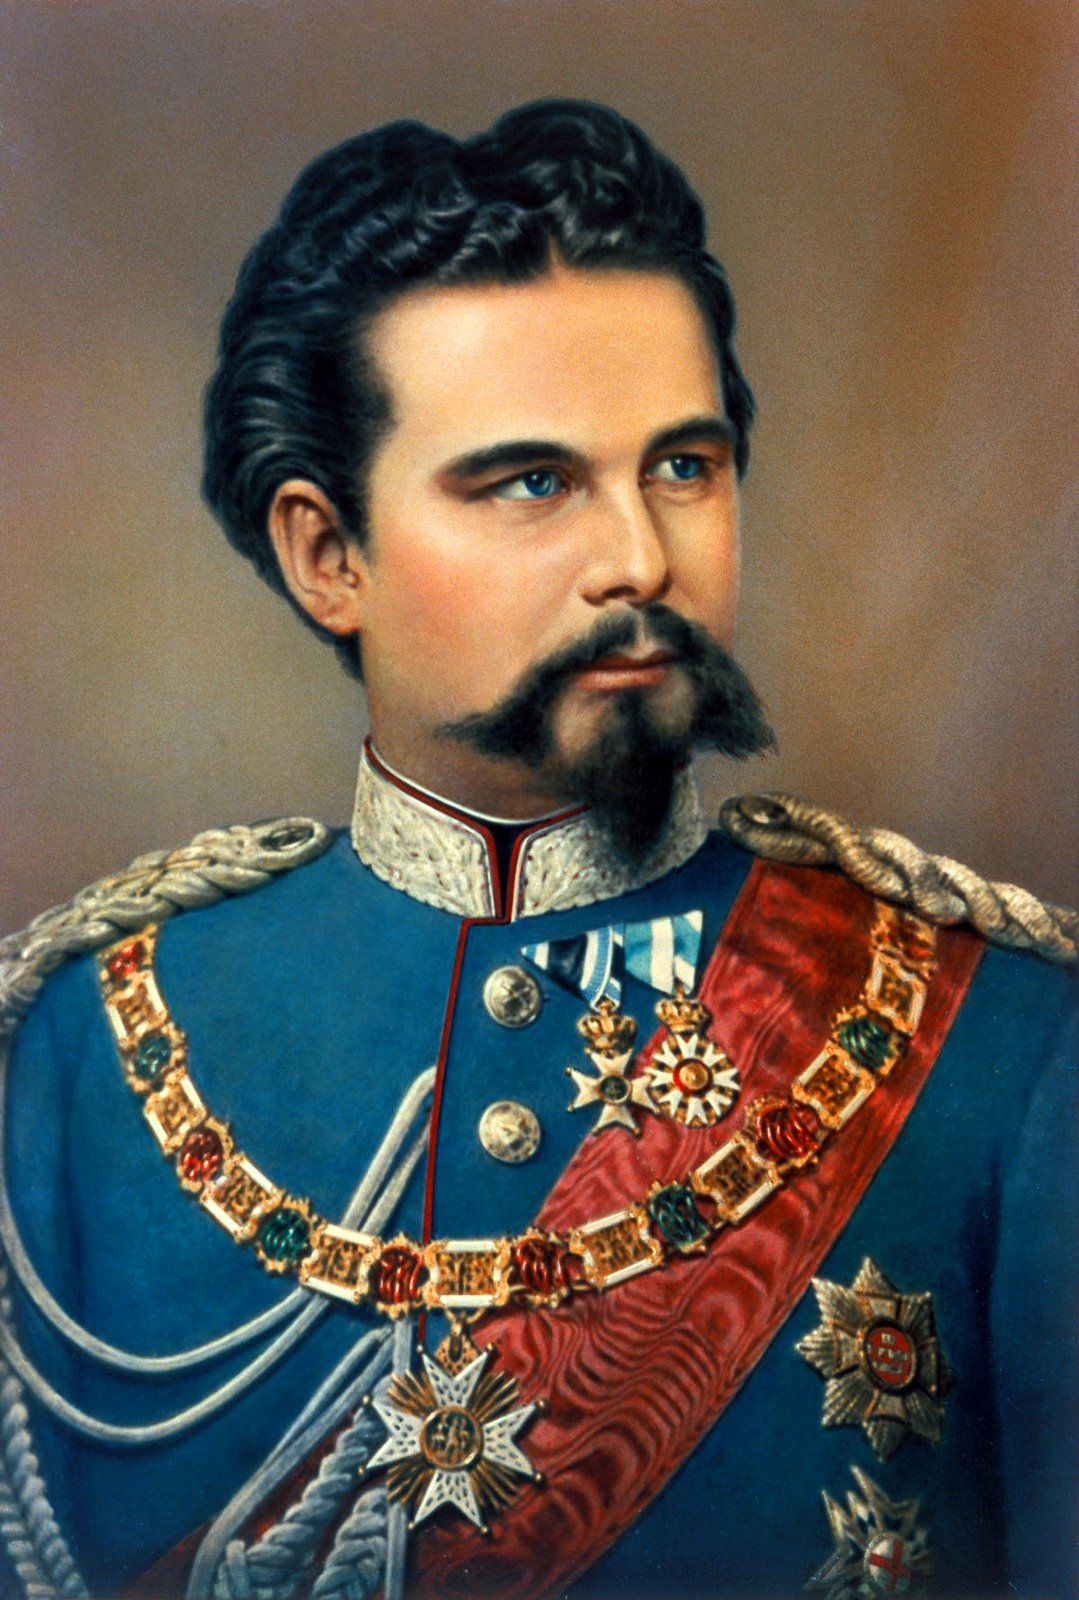
\includegraphics[height=0.3\textheight]{LudwigII}
    \caption{König Ludwig II}
\end{figure}


\begin{figure}[htb]
    \centering
    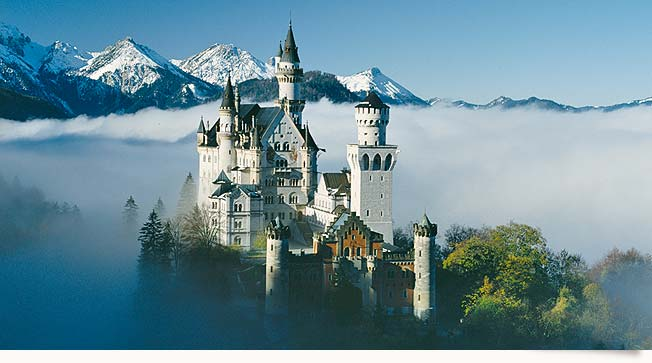
\includegraphics[height=0.3\textheight]{neuschwanstein_23}
    \caption{König Ludwig II}
\end{figure}

